\documentclass[12pt]{article}
\usepackage[spanish,mexico]{babel}
	\selectlanguage{spanish}
\usepackage{graphicx}
\usepackage{amsmath}
\usepackage{wrapfig}
\usepackage{subcaption}
\usepackage{array}
\usepackage{color}
\usepackage[dvipsnames]{xcolor}

\usepackage{float}
\usepackage{multicol}
\usepackage{geometry}
\usepackage{hyperref}
\usepackage[utf8]{inputenc}

\newgeometry{top=2cm}
\definecolor{labelcolor}{RGB}{100,0,0}

\title{Actividad 11: Apocalipsis Zombie}
\author{Ana Gabriela Carretas Talamante}
\date{01 de mayo de 2016}

\begin{document}
\maketitle
\section{Introducción}
Un zombie es una persona que ha perdido su sentido de conciencia e identidad, y que solo le importa la destrucción (y en veces el consumo) de cualquier humano alrededor, sin importar la circunstancias o el costo del mismo. Técnicamente, los verdaderos zombies son muertos reanimados con un instinto asesino de propagar el estado de ``zombiecidad'' \cite{ZP}.

\begin{figure}[H]
\centering
 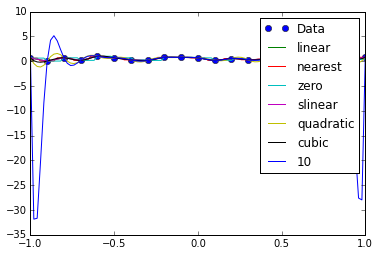
\includegraphics[width=12cm]{1}
 \caption{Zombies subiendo una muralla en la película de ``Guerra Mundial Z'' \cite{F}.}
\end{figure}

En la presente actividad se realizan diferentes gráficas que ilustran las poblaciones de humanos y zombies en diferentes casos de propagación. Cada modelo involucra distintos tipos de población; por practicidad, mencionamos estos a continuación.

\subsection{Tipos de población}
\begin{itemize}
\item \textbf{Susceptibles (S):} Población humana que puede infectarse, morir o convertirse en zombie.
\item \textbf{Zombie (Z):} Población zombieficada.
\item \textbf{Removidos (R):} Población que ha muerto, pero puede volverse zombie (los zombies al ser removidos no pueden resucitar).
\item \textbf{Infectados (I):} Población que tras estar infectada puede morir (pasar a los removidos) o convertirse en zombie.
\item \textbf{Cuarentena (Q):} Población infectada, zombie o removida que no puede infectar a susceptibles mientras se mantenga en cuarentena.
\end{itemize}

Ahora, comenzaremos a describir cada caso propuesto por el artículo \cite{Z}, y con ayuda del tutorial \cite{ZSC}, poder graficar cada uno.

\section{Modelo básico}
En este modelo participan tres clases de población: S, R, Z. El diagrama de flujo de población se presenta en la figura \ref{SZR}; como se puede notar, aparece dentro del modelo el uso de diversos parámetros, asociados con este mismo flujo poblacional.

\begin{figure}[H]
\centering
 \includegraphics[width=9cm]{SZR}
 \caption{Modelo básico \cite{Z}.}
 \label{SZR}
\end{figure}

\subparagraph*{Parámetros utilizados por el modelo}
\begin{itemize}
\item $\delta$: Tasa de muertes humana.
\item $\alpha$: Tasa de muertes zombie.
\item $\zeta$: Tasa de transimisón zombie-muerto.
\item $\beta$: Tasa de transmisión zombie-sano.
\item $\prod$: Tasa de natalidad humana.
\end{itemize}

\subsection*{Programa: Modelo básico.}

{\color{RoyalPurple}\begin{verbatim}

# Modelo Basico
import numpy as np
import matplotlib.pyplot as plt
from scipy.integrate import odeint


P = 0       # Tasa de natalidad humana
d = 0.0001  # Tasa de muertes humana
B = 0.0095  # Tasa de transmisión zombie-sano
G = 0.0001  # Tasa de transimisón zombie-muerto
A = 0.005   # Tasa de muertes zombie

#Planteando el SED
def f(y, t):
    Si = y[0]
    Zi = y[1]
    Ri = y[2]
    
    #Las ecuaciones modelo por el articulo
    f0 = P - B*Si*Zi - d*Si
    f1 = B*Si*Zi + G*Ri - A*Si*Zi
    f2 = d*Si + A*Si*Zi - G*Ri
    return [f0, f1, f2]

#Condiciones iniciales
S0 = 500.                   # Sanos
Z0 = 0                      # Zombies
R0 = 0                      # Muertos
y0 = [S0, Z0, R0]           # Vector de CI
t  = np.linspace(0, 20, 1000)       # Tiempo desde la infeccion

#Resolviendo el SED
soln = odeint(f, y0, t)
S = soln[:, 0]
Z = soln[:, 1]
R = soln[:, 2]

#Graficando suave
plt.grid()
plt.plot(t, S,"m",label='Sanos')
plt.plot(t, Z,"g", label='Zombies')
plt.xlabel('Dias desde la infeccion')
plt.ylabel('Poblacion')
plt.xlim(0,20)
plt.ylim(-10,550)
plt.title('Apocalipsis zombie: Modelo Basico')
plt.legend(loc=0)



#Pa' guardar la foto sin problemas
fig = matplotlib.pyplot.gcf()
fig.set_size_inches(10.5,5.5)
fig.savefig('Z1.png',dpi=100)
\end{verbatim}}

\subsection*{Gráficas obtenidas}

\begin{figure}[H]
    \centering
    \begin{subfigure}[b]{\textwidth}
    \centering
        \includegraphics[width=14cm]{Z0}
        \caption{Modelo básico con 0 tasa de transmición zombie-humano.}
    \end{subfigure}
    \begin{subfigure}[b]{\textwidth}
    \centering
        \includegraphics[width=14cm]{Z1}
        \caption{Modelo básico con cierta tasa de transmisión infecciosa.}
    \end{subfigure}
    \caption{Dos versiones del modelo básico.}
\end{figure}

\section{Modelo con infección latente}
En este modelo participan cuatro clases de población: S, I, Z, R. El diagrama de flujo de población se presenta en la figura \ref{SIZR}.

\begin{figure}[H]
\centering
 \includegraphics[width=9cm]{SIZR}
 \caption{Modelo con infección latente \cite{Z}.}
 \label{SIZR}
\end{figure}

\subparagraph*{Parámetros utilizados por el modelo}
\begin{itemize}
\item $\delta$: Tasa de muertes humana.
\item $\alpha$: Tasa de muertes zombie.
\item $\zeta$: Tasa de transimisón zombie-muerto.
\item $\beta$: Tasa de transmisión zombie-sano.
\item $\rho$: Tasa de transmisión zombie-infectado.
\item $\prod$: Tasa de natalidad humana.
\end{itemize}

\subsection*{Programa: Modelo infección latente.}

{\color{RedViolet}\begin{verbatim}
#Modelo con Infeccion Latente
import numpy as np
import matplotlib.pyplot as plt
from scipy.integrate import odeint

P = 0       # Tasa de natalidad humana
d = 0.0001  # Tasa de muertes humana
B = 0.0095  # Tasa de transmisión zombie-sano
G = 0.0001  # Tasa de transimisón zombie-muerto
A = 0.0001  # Tasa de muertes zombie
rho = 0.3     # Tasa de transmisión zombie-infectado




#Planteando el SED
def f(y, t):
    Si = y[0]
    Ii = y[1]
    Zi = y[2]
    Ri = y[3]
  
    #Las ecuaciones modelo por el articulo
    f0 = P - B*Si*Zi - d*Si
    f1 = B*Si*Zi - rho*Ii - d*Ii
    f2 = rho*Ii + G*Ri - A*Si*Zi
    f3 = d*Si + d*Ii + A*Si*Zi - G*Ri
    return [f0, f1, f2, f3]

#Condiciones iniciales
S0 = 500.                   # Sanos
I0 = 1                      # Infectados
Z0 = 0                      # Zombies
R0 = 0                      # Muertos
y0 = [S0, I0, Z0, R0]       # Vector de CI
t  = np.linspace(0, 50, 1000)       # Tiempo desde la infeccion

#Resolviendo el SED
soln = odeint(f, y0, t)
S = soln[:, 0]
I = soln[:, 1]
Z = soln[:, 2]
R = soln[:, 3]

#Graficando suave
plt.grid()
plt.plot(t, S,"m",label='Sanos')
plt.plot(t, Z,"g", label='Zombies')
plt.xlabel('Dias desde la infeccion')
plt.ylabel('Poblacion')
plt.xlim(0,50)
plt.ylim(-10,550)
plt.title('Apocalipsis zombie: Modelo con Infeccion Latente')
plt.legend(loc=5)

#Pa' guardar la foto sin problemas
fig = matplotlib.pyplot.gcf()
fig.set_size_inches(10.5,5.5)
fig.savefig('Z2.png',dpi=100)
\end{verbatim}}

\subsection*{Gráficas obtenidas}

\begin{figure}[H]
\centering
 \includegraphics[width=15cm]{Z2}
 \caption{Modelo con infección latente.}
\end{figure}

\section{Modelo con cuarentena}
En este modelo participan cuatro clases de población: S, I, Z, R, Q. El diagrama de flujo de población se presenta en la figura \ref{SIZRQ}.

\begin{figure}[H]
\centering
 \includegraphics[width=9cm]{SIZRQ}
 \caption{Modelo con cuarentena \cite{Z}.}
 \label{SIZRQ}
\end{figure}

\subparagraph*{Parámetros utilizados por el modelo}
\begin{itemize}
\item $\delta$: Tasa de muertes humana.
\item $\alpha$: Tasa de muertes zombie.
\item $\gamma$: Tasa de muertes en cuarentena.
\item $\zeta$: Tasa de transimisón zombie-muerto.
\item $\beta$: Tasa de transmisión zombie-sano.
\item $\rho$: Tasa de transmisión zombie-infectado.
\item $\kappa$: Tasa de infectados en cuarentena.
\item $\sigma$: Tasa de zombies en cuarentena.
\item $\prod$: Tasa de natalidad humana.
\end{itemize}

\subsection*{Programa: Modelo con cuarentena.}

{\color{Fuchsia}\begin{verbatim}
#Modelo con Cuarentena
import numpy as np
import matplotlib.pyplot as plt
from scipy.integrate import odeint

P = 0         # Tasa de natalidad humana
d = 0.0001    # Tasa de muertes humana
B = 0.0095    # Tasa de transmisión zombie-sano
G = 0.0001    # Tasa de transimisón zombie-muerto
A = 0.0001    # Tasa de muertes zombie
rho = 0.5     # Tasa de transmisión zombie-infectado
k = 0.001     # Tasa de infectados en cuarentena
sigma = 0.009 # Tasa de zombies en cuarentena
Ga = 0.004    # Tasa de muertes en cuarentena

#Planteando el SED
def f(y, t):
    Si = y[0]
    Ii = y[1]
    Zi = y[2]
    Ri = y[3]
    Qi = y[4]
    
    #Las ecuaciones modelo por el articulo
    f0 = P - B*Si*Zi - d*Si
    f1 = (B*Si*Zi)-(rho*Ii)-(d*Ii)-(k*Ii)
    f2 = (rho*Ii) + (G*Ri)-(A*Si*Zi)-(sigma*Zi)
    f3 = (d*Si) + (d*Ii) + (A*Si*Zi)-(G*Ri)+(Ga*Qi)
    f4 = (k*Ii)+(sigma*Zi)-(Ga*Qi)
    return [f0, f1, f2, f3, f4]
  
  
#Condiciones iniciales
S0 = 500.                   # Sanos
I0 = 100                    # Infectados
Z0 = 0                      # Zombies
R0 = 0                      # Muertos
Q0 = 0

y0 = [S0, Z0, R0, I0, Q0]       # Vector de CI
t  = np.linspace(0, 100, 1000)       # Tiempo desde la infeccion

#Resolviendo el SED
soln = odeint(f, y0, t)
S = soln[:, 0]
I = soln[:, 1]
Z = soln[:, 2]
R = soln[:, 3]
Q = soln[:, 4]

#Graficando suave
plt.grid()
plt.plot(t, S,"m",label='Sanos')
plt.plot(t, Z,"g", label='Zombies')
plt.xlabel('Dias desde la infeccion')
plt.ylabel('Poblacion')
plt.xlim(0,100)
plt.ylim(-10,550)
plt.title('Apocalipsis zombie: Modelo con Cuarentena')
plt.legend(loc=5)

#Pa' guardar la foto sin problemas
fig = matplotlib.pyplot.gcf()
fig.set_size_inches(10.5,5.5)
fig.savefig('Z3.png',dpi=100)
\end{verbatim}}

\subsection*{Gráficas obtenidas}

\begin{figure}[H]
\centering
 \includegraphics[width=15cm]{Z3}
 \caption{Modelo con cuarentena.}
\end{figure}


\section{Modelo con cura}
En este modelo participan cuatro clases de población: S, I, Z, R. El diagrama de flujo de población se presenta en la figura \ref{SIZRc}.

\begin{figure}[H]
\centering
 \includegraphics[width=9cm]{SIZRc}
 \caption{Modelo con cura \cite{Z}.}
 \label{SIZRc}
\end{figure}

\subparagraph*{Parámetros utilizados por el modelo}
\begin{itemize}
\item $\delta$: Tasa de muertes humana.
\item $\alpha$: Tasa de muertes zombie.
\item $\zeta$: Tasa de transimisón zombie-muerto.
\item $\beta$: Tasa de transmisión zombie-sano.
\item $\rho$: Tasa de transmisión zombie-infectado.
\item $c$: Tasa de cura de zombies.
\item $\prod$: Tasa de natalidad humana.
\end{itemize}

\subsection*{Programa: Modelo con cura.}

{\color{BlueViolet}\begin{verbatim}
#Modelo con Cura
import numpy as np
import matplotlib.pyplot as plt
from scipy.integrate import odeint

P = 0       # Tasa de natalidad humana
d = 0.0001  # Tasa de muertes humana
B = 0.0095  # Tasa de transmisión zombie-sano
G = 0.0001  # Tasa de transimisón zombie-muerto
A = 0.0001  # Tasa de muertes zombie
rho = 0.3   # Tasa de transmisión zombie-infectado
c = 0.2     # Tasa de cura de zombies

#Planteando el SED
def f(y, t):
    Si = y[0]
    Ii = y[1]
    Zi = y[2]
    Ri = y[3]
  
    #Las ecuaciones modelo por el articulo
    f0 = P - B*Si*Zi - d*Si + c*Zi
    f1 = B*Si*Zi - rho*Ii - d*Ii
    f2 = rho*Ii + G*Ri - A*Si*Zi - c*Zi
    f3 = d*Si + d*Ii + A*Si*Zi - G*Ri
    return [f0, f1, f2, f3]

#Condiciones iniciales
S0 = 500.                   # Sanos
I0 = 4                      # Infectados
Z0 = 0                      # Zombies
R0 = 0                      # Muertos
y0 = [S0, I0, Z0, R0]       # Vector de CI
t  = np.linspace(0, 100, 1000)       # Tiempo desde la infeccion



#Resolviendo el SED
soln = odeint(f, y0, t)
S = soln[:, 0]
I = soln[:, 1]
Z = soln[:, 2]
R = soln[:, 3]

#Graficando suave
plt.grid()
plt.plot(t, S,"m",label='Sanos')
plt.plot(t, Z,"g", label='Zombies')
plt.xlabel('Dias desde la infeccion')
plt.ylabel('Poblacion')
plt.xlim(0,100)
plt.ylim(-10,550)
plt.title('Apocalipsis zombie: Modelo con Cura')
plt.legend(loc=0)

#Pa' guardar la foto sin problemas
fig = matplotlib.pyplot.gcf()
fig.set_size_inches(10.5,5.5)
fig.savefig('Z4.png',dpi=100)
\end{verbatim}}

\subsection*{Gráficas obtenidas}

\begin{figure}[H]
\centering
 \includegraphics[width=15cm]{Z4}
 \caption{Modelo con cura.}
\end{figure}


\pagebreak

\begin{thebibliography}{6}

\bibitem{ZP}
Zombiepedia.
\emph{Types of Zombies}. Recuperado en mayo de 2016 de \url{http://zombie.wikia.com/wiki/Types_of_Zombies}

\bibitem{F}
Recuperado en mayo de 2016 de \url{http://a69.g.akamai.net/n/69/10688/v1/img5.allocine.fr/acmedia/medias/nmedia/18/83/67/73/20517467.jpg}

\bibitem{Z}
Munz P., Hudea, I., Imad, J., Smith, R.J.
\emph{When Zombies Attack!: Mathematical Modelling of an Outbreak of Zombie Infection}. Recuperado en mayo de 2016 de \url{http://mysite.science.uottawa.ca/rsmith43/Zombies.pdf}

\bibitem{ZSC}
SciPy Cookbook.
\emph{Modeling a Zombie Apocalypse}. Recuperado en mayo de 2016 de \url{http://scipy-cookbook.readthedocs.io/items/Zombie_Apocalypse_ODEINT.html}

\bibitem{FC}
Lizárraga, C.
\emph{Actividad 11 (2016-1)}. Recuperado en mayo de 2016 de \url{http://computacional1.pbworks.com/w/page/107502219/Actividad\%2011\%20(2016-1)}

\end{thebibliography}

\end{document}


